\section{Reinforcement Learning}
Reinforcement learning \cite{sutton2018reinforcement} describes a solution to a Markov Decision Process 
with the goal of finding a policy that maximizes the sum of rewards \cite{huys2014reward}.
%
The agent learns an optimal (or nearly optimal) policy for the environment \cite{russell2002artificial}
through a series of reinforcements (rewards or penalties) that provide a quality of its behavior.

\begin{figure}[ht]
    \centering
    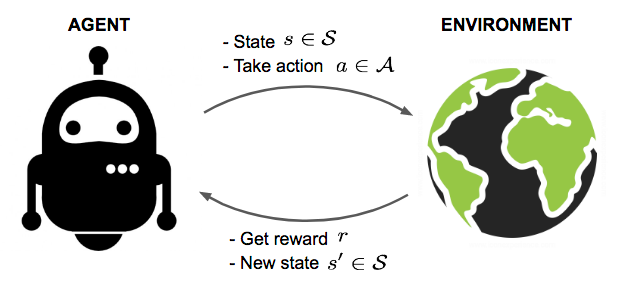
\includegraphics[scale=0.4]{images/RL_illustration.png}
    \caption{Simple diagram of the functioning of an RL system.}
    \label{fig:RL_illustration}
\end{figure}

\newpage
\noindent
Reinforcement learning is divided in two approaches:
\begin{itemize}
    \item \textbf{Model-based}:
    The agent uses a transition model of the environment to help interpret the reward signals and to make decisions about how to act \cite{russell2021artificial}.    
    \item \textbf{Model-free}:
    The agent learns the consequences of his actions through experience in order to refine his policy.
\end{itemize}


\subsection{Q-Learning}
Q-learning \cite{watkins1992q} is a model-free reinforcement learning algorithm which estimate a value for each (state, action) pair
and with these estimated values compute a policy that can maximize the expected discounted reward.

Given S a set of states of the environments, A a set of agents's possible actions,
$\pi$ : SxAxS $\rightarrow$ [0, 1] a function which gives the probability of reaching state s' while agent is in the state s and perform the action a,
r : SxAxS $\rightarrow$ $\mathbb{R}$ a function which gives the amount of reward the agent will receive when perform the action a while in state s and move to state s',
the cumulative discounted reward can be defined as $R_t = \sum_{i=0}^{\infty} \gamma^i r_{t+k+1}$
where $\gamma$ $\in$ [0, 1] is the discount factor which makes futures rewards less valuable than the current ones.

The algorithm, therefore, has a function that calculates the quality of a pair (state, action): $Q:S\times A\to {\mathbb  {R}}$.
\begin{equation*}
    Q(s_t, a_t) \leftarrow Q(s_t, a_t) + \alpha [r_{t+1} + \gamma \max_a Q(s_{t+1}, a) - Q(s_t, a_t)] 
\end{equation*}
where $\alpha$ is the learning rate.

``an agent tries an action at a particular state, and evaluates its consequences in terms of the immediate reward or penalty
it receives and its estimate of the value of the state to which it is taken''\cite{watkins1992q}.
``By trying all actions in all states repeatedly, it learns which are best overall, judged by long-term discounted reward''\cite{watkins1992q}.

Given a finite Markov Decision Process, infinite exploration time and a partly-random policy
the Q-learning algorithm is able to learn an optimal action-selection policy.

A problem of this method is the limitation of the state-action space required, that can be partially solved with an approximation function.
instead of storing each Q-values a mapping function could be learned to map a state-action pair to their respective Q-value.

\subsection{SARSA}
SARSA algorithm \cite{qiang2011reinforcement} is a variation of the Q-learning algorithm.
Its name come from $(s, a, r, s', a')$, that are $(state, action, reward, state', action')$, and they are used to compute the update.

An algorithm has an "Off-Policy" technique if it learns the value function according to the action derived from another policy. On the other hand, it called "On-Policy" if it learns the value function according to the current action derived from the current policy.
Q-learning has an Off-Policy technique while SARSA has an On-Policy one.

The update formula of SARSA is similar to the one used by the Q-learning: 
\begin{equation*}
    Q(s_t, a_t) \leftarrow Q(s_t, a_t) + \alpha [r_{t+1} + \gamma Q(s_{t+1}, a) - Q(s_t, a_t)]    
\end{equation*}

This means that SARSA updates the state based on the action taken, while Q-learning updates following the optimal policy.
Suppose to be in a "cliff world", where the agent has to walk from the starting cell to the goal cell along the edge of a cliff without falling off. Q-learning, following the optimal policy, would tend to be close to the edge of the cliff while SARSA would prefer a "safer" path.

\begin{figure}[ht]
    \centering
    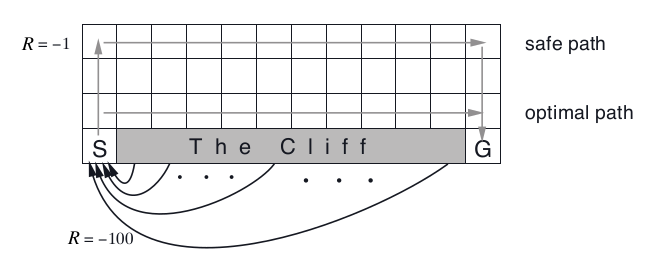
\includegraphics[scale=0.4]{images/cliff_word.png}
    \caption{Image to show the difference between SARSA and Q-learning in a "cliff word".}
\end{figure}

\subsubsection{Temporal Difference}

\subsection{Deep Reinforcement Learning}
When there are too many states and actions, more memory and more time are required for learning.
To solve these problems it is possible to use approximation functions.
The function can be linear \cite{melo2008analysis} or non-linear as in the case of neural networks.

\vspace*{4mm}
\noindent
"Deep Reinforcement Learning: Pong from Pixels" \cite{karpathy2016deep} show how applying Deep Reinforcement Learning for the game of pong leads to the best results.

The policy function, or policy network, used to decide what to do based on the current state, is a fully connected neural network with n hidden layers, which is why this method is called Deep RL. In the papers frame image of the game is taken as input, in which each pixel corresponds to a single input neuron, and returns a number between 0 and 1 which can be seen as the probability to win with a given action (e.g. left). If the number is greater than 0.5 we go to the left, otherwise we go to the right. If it is 0.5, a random choice is made. To do this, the output neuron has a sigmoid function \cite{mnih2013playing}\cite{karpathy2016deep}.
Since politics generates probability, this politics is stochastic.

\begin{figure}[ht]
  \centering
  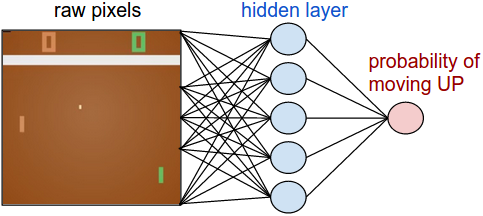
\includegraphics[scale=0.4]{images/DRL_network.png}
  \caption{Simple image of the policy network of an Deep RL system.}
  \label{fig:DRL_network}
\end{figure}

Therefore fully connected neural networks have been replaced by convolutional neural networks and in ”Playing Atari
with Deep Reinforcement Learning” \cite{mnih2013playing} Deep Q Networks(DQN) were introduced.

A DQN is a CNN adapted for RL used as a function approximator to estimate the Q-values, where the inputs are images and the outputs depends on the task's number of actions.
The loss is defined as the mean squared error between the Q-value target and the network's predicted at step $i$.
\begin{equation*}
    L(\theta_i) \leftarrow \mathbb{E}_{s, a, r, s'} [((r + \gamma \max_{a'} Q(s', a'; \theta_i)) - Q(s, a; \theta_{i-1}))^2]    
\end{equation*}
where $s$ is the current state, $s'$ the next state, a the current action selected by the $\epsilon$-greedy policy, $r$ the immediate reward and $\theta$ are the network parameters.

To avoid computing the full expectation in the DQN loss, we can minimize it using stochastic gradient descent

Experience Replay is a technique introduced in The Atari DQN work to make the network updates more stable.
This method At each time step of data collection, add the transitions to a circular buffer called the replay buffer.

Given a random batch of transitions $(s, a, r, s')$ from the replay buffer we can calculate the loss at step $i$ as the following formula:
\begin{equation*}
    L(\theta_i) \leftarrow ((r + \gamma \max_{a'} Q(s', a'; \theta_i)) - Q(s, a; \theta_{i-1}))^2    
\end{equation*}

A very big advantage that Deep RL offers instead of other input representation,
is that it can handle unseen states well \cite{mnih2013playing} \cite{karpathy2016deep}.

This is because a large portion of pixels could be similar to an image already seen and on which the model has been trained, so the network is likely to produce a similar prediction to the image seen previously. Instead, algorithms like MDP behave randomly in these cases.

Generally, to facilitate learning, pre-processing is applied.
An image can then be cropped to eliminate those pixels that are not needed for prediction, such as the scoreboard. Other things that can help are grayscaling the image and reducing image resolution \cite{mnih2013playing}.
